\hypertarget{modelling-reactive-behavior-notation---pulse-cast-interaction}{%
\section{Modelling Reactive Behavior Notation -
Pulse-Cast-Interaction}\label{modelling-reactive-behavior-notation---pulse-cast-interaction}}

Used for synchronous Interaction between reactive-objects.

\begin{figure}[H]
\centering
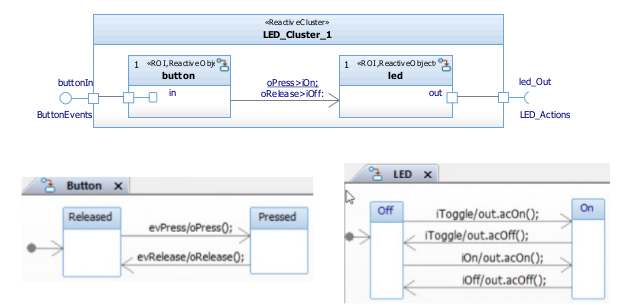
\includegraphics[width=1\textwidth]{figures/pulseCastOverview.png}
\caption{Pulse Cast Overview}
\end{figure}

\hypertarget{mechanism}{%
\subsection{Mechanism}\label{mechanism}}

\begin{itemize}
\tightlist
\item
  Out-pulses may be generated on a state-transition
\item
  Pulses are transmitted at the end of a transition, i.e.~the sender is
  already in the new state
\item
  On transmission, out-pulses of the sender are translated into
  in-pulses for the receiver
\item
  The pulse-cast-connection defines receiver and translation of
  out-pulses to in-pulses
\item
  An out-pulse may be translated in many different in-pulses for
  different receivers - they are transmitted according to the cast-order
\item
  An in-pulse may trigger a state-transition of the receiver object
\item
  Unhandled in-pulses, will be lost
\end{itemize}

\begin{figure}[H]
\centering
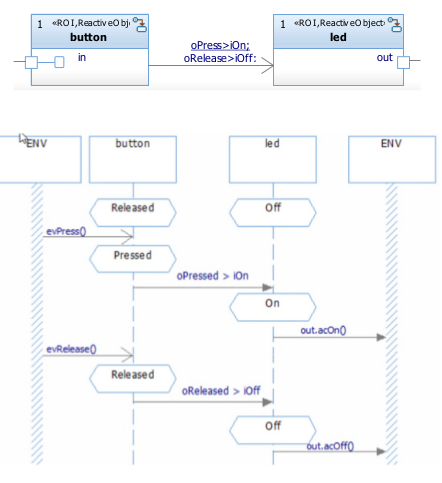
\includegraphics[width=0.65\textwidth]{figures/castsExample.png}
\caption{Casts Example}
\end{figure}

\hypertarget{cast-order}{%
\subsection{Cast-Order}\label{cast-order}}

\begin{itemize}
\tightlist
\item
  Defines the transmission order of pulses in a multi-cast situation
\item
  Is defined by a number at the beginning of the pulse-cast connection
  label
\end{itemize}

\hypertarget{three-variants}{%
\subsubsection{Three Variants:}\label{three-variants}}

P, Q, S, T, R, U (deep-first)\\
P, Q, R, S, T, U (left-first) / (right first)\\
P, Q, S, R, U, T (irregular)

\begin{figure}[H]
\centering
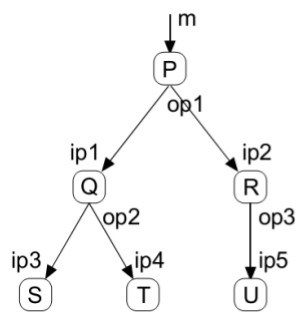
\includegraphics[width=0.25\textwidth]{figures/pulse-cast-chains.png}
\caption{Pulse Cast Chaines}
\end{figure}

\begin{itemize}
\tightlist
\item
  Wir können selbst entscheiden, ob wir nur die Input-Cast beim Sequence
  Diagram oder auch der Output-Cast (gesamte Translation) hinschreiben.
\item
  \textbf{Wir müssen an der MEP mindestens 2 Sequenz-Diagramme
  zeichnen.}
\end{itemize}

\begin{figure}[H]
\centering
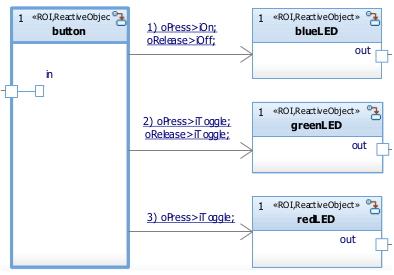
\includegraphics[width=0.7\textwidth]{figures/LED-Cluster.png}
\caption{LED Cluster}
\end{figure}

\begin{figure}[H]
\centering
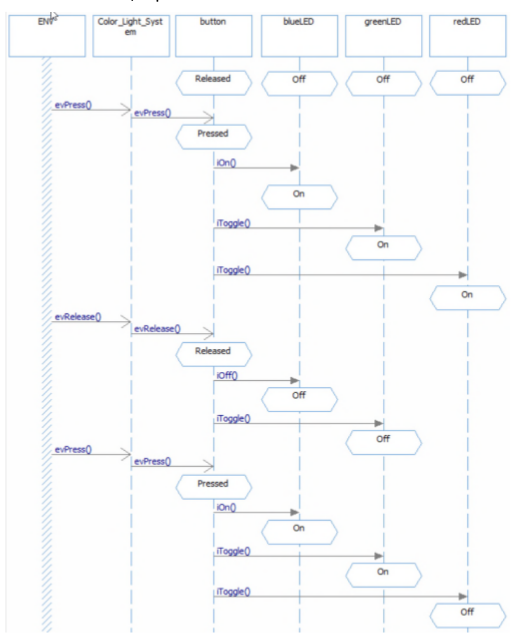
\includegraphics[width=0.82\textwidth]{figures/sequenceDiagramExample.png}
\caption{Sequence Diagram Example}
\end{figure}

\textbf{Reactive-Object-Step}:
\begin{itemize}
    \item Asynchronious Event from outside the cluster
    \item Triggered by a message or an In-Pulse
\end{itemize}

\textbf{Cluster Step}: 
\begin{itemize}
    \item Synchronious Events within the cluster
    \item Triggered by a message to the cluster
     \item The sequence is not interruptible $\Rightarrow$ Run to Completion
     \item every cluster-step must have an end (no infinite cluster steps)
\end{itemize}

\clearpage